% -------------------------
% INTRODUCTION
% -------------------------

\graphicspath{{./\figurefolder/2ResearchContext/}}
% ----------------------------------------------------------------------------------------------------
% 0. Front Matter
% ----------------------------------------------------------------------------------------------------

\chapter{Research Context and Literature Review on Structural Cooperative Robotic Fabrication} \label{chap:2_context}

\thispagestyle{empty}

\vfill 
\section*{\normalsize\textmd{This chapter is based on the following publication:}}
    \vspace{-0.3cm}\noindent
    \textbf{Bruun, E. P. G.}, Parascho, S., \& Adriaenssens, S. (2024). Cooperative Robotic Fabrication for a Circular Economy. In A Circular Built Environment in the Digital Age (pp. 129–149). Springer Cham. https://doi.org/10.1007/978-3-031-39675-5\_8

\section*{\normalsize\textmd{Contributor roles in publication:}}
    \vspace{-0.3cm}\noindent
    - Bruun: Conceptualization, Methodology, Investigation, Writing (Original Draft), Writing (Review and Editing), Visualization\\
    - Parascho \& Adriaenssens: Writing (Review and Editing), Supervision, Funding Acquisition \\
    
% ----------------------------------------------------------------------------------------------------
% 1. Introduction
% ----------------------------------------------------------------------------------------------------
\newpage

\section{What is Cooperative Robotic Behaviour?} \label{sec:01_intro}
    Robotic fabrication (RF) refers to any fabrication process that is completed with some degree of automation. Cooperative Robotic Fabrication (CRF) is a subset of RF and can be thought of as any process where the robotic agents are specifically coordinated to accomplish tasks that would not be possible if the robots were working alone. Cao et al. state that ``a multiple robot system displays cooperative behaviour if, due to [the mechanism of cooperation], there is an increase in the total utility of the system'' \cite[p.8]{cao_cooperative_1997}. Thus, cooperative robotic cells can fall under the category of either multi-arm individual robots, multiple single-arm robots, mechanical hands with independently controllable fingers, or a combination of these, working together in a synchronous fashion \citep{ranky_collaborative_2003, liu_quality_2004}.
    
    A single robotic agent, regardless of physical or digital complexity, is naturally limited in the type and number of actions it can simultaneously execute. Only in multi-robotic fabrication (MRF), where multiple agents are placed together in a work cell, does it become possible to unlock the potential of collective behaviour to achieve more complex outputs. All MRF setups exhibit some form of collective behaviour, but while cooperative behaviour is subset of collective behaviour (i.e., $CRF \subseteq MRF$), the converse is not true (i.e., $MRF \nsubseteq CRF$). A CRF process entails further utility beyond the collective behaviour that comes from a basic implementation of MRF. This hierarchy is illustrated in \Cref{fig:01}, where the output of an MRF setup is defined as scaling linearly with the number of agents to produce more of the same output (i.e., several robots working in parallel), as opposed to a CRF process where the output is uniquely contingent on all the agents working together.

    \begin{figure}[ht]
    	\centering
    	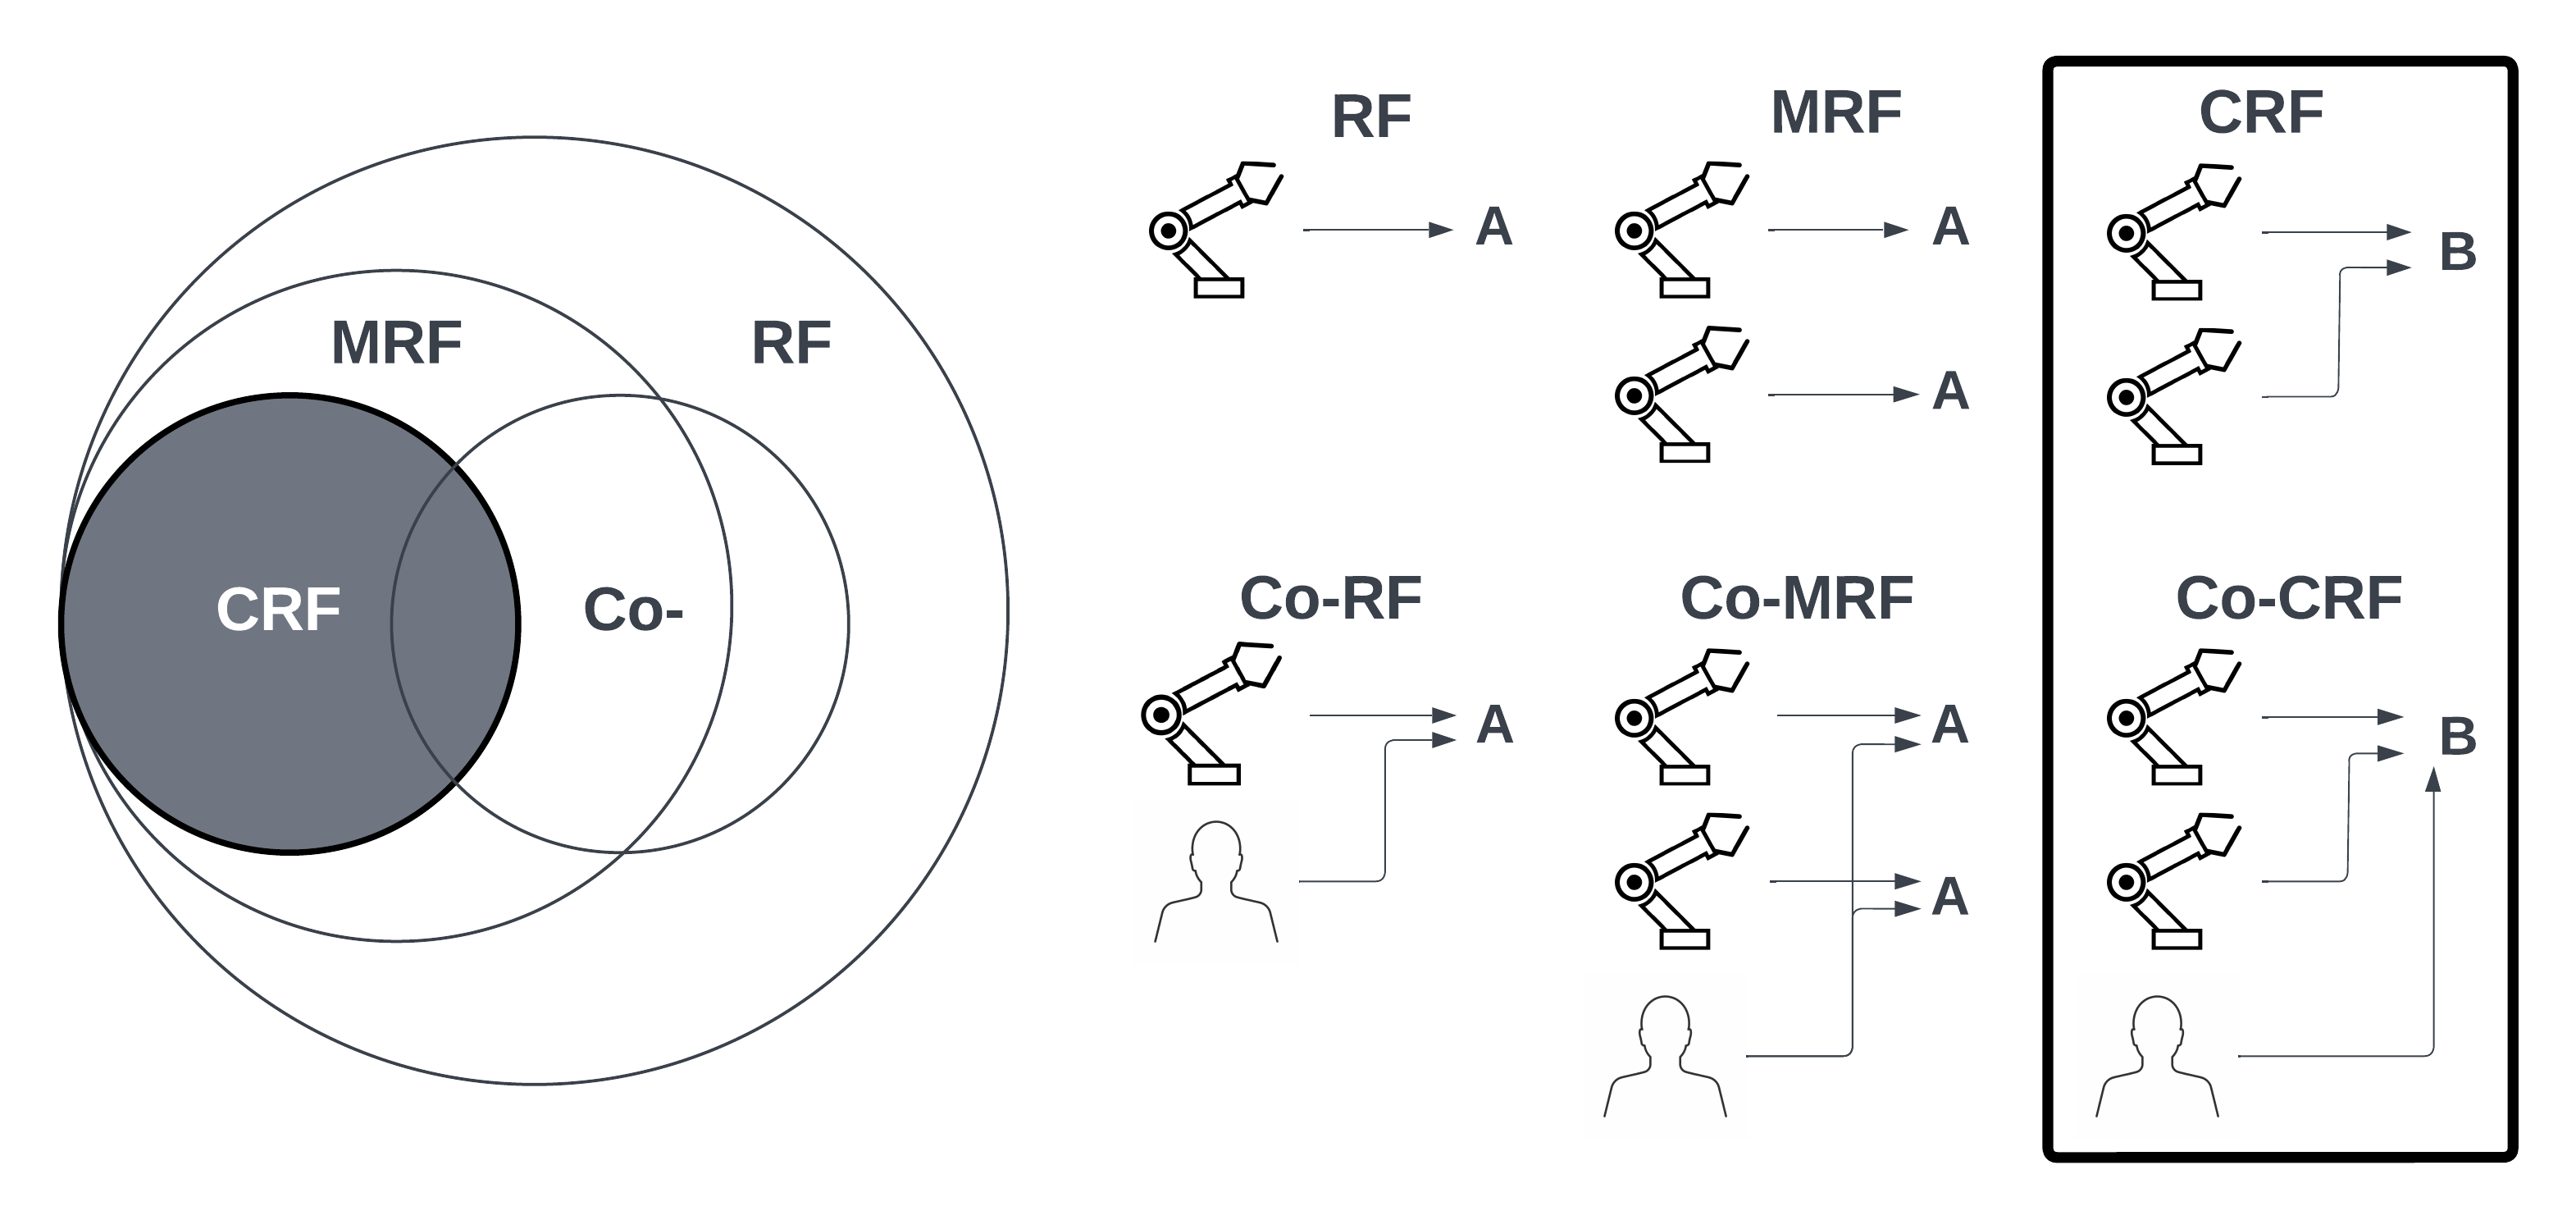
\includegraphics [trim={0cm 0.0cm 0cm 0.0cm}, clip, width=0.99\linewidth]{coop_definition} %tight
    	\caption{Cooperative robotic fabrication as situated in the overall robotic setup hierarchy (RF = robotic fabrication, MRF = multi-robotic fabrication, CRF = cooperative robotic fabrication, Co = collaborative). A setup is cooperative, if by the process of cooperation, a novel output is made possible (i.e., B), as opposed to a basic MRF process which only allows more of the same output to be created in parallel (i.e., A)}
    	\label{fig:01} 
    \end{figure}   
    
    Another important distinction is between the terms cooperative and collaborative, which are commonly used interchangeably to describe multi-agent robotic processes in the literature. To avoid ambiguity, collaborative is within this dissertation only used for a process where robot(s) work together with, or alongside, human operators. Collaborative processes exist across the entire RF hierarchy illustrated in \Cref{fig:01}. For example, collaborative processes are possible with a human working with a single robot (Co-RF, as in \cite{asadi_pictobot_2018}), with multiple robots in series on an assembly line (Co-MRF, as in \cite{weckenborg_balancing_2020}), or to complement the cooperative function of multiple robots (Co-CRF, as in \cite{bruun_humanrobot_2020}).
    
\subsection{Broad Applications} \label{sec:1_apps}
    Alongside applications in the built environment, which are specifically discussed in \Cref{sec:02_built}, CRF is utilised in many industries when flexible manufacturing systems are necessary or where tasks occur in poorly structured environments \citep{caccavale_cooperative_2016}. In generic manufacturing applications, CRF processes have a conceptual advantage over single robot processes with their ability to distribute the work among several potentially smaller robots and thus better control the internal forces, torques and displacements associated with a payload \citep{montemayor_decentralized_2005}. In addition, CRF processes also allow for improved robustness against work interruptions through redundancy in the functions of the robots, improved flexibility through the ability to reconfigure a fabrication cell to fit different conditions, and improved task precision through the ability to dexterously grasp and then manipulate an object \citep{gudino-lau_dynamic_2005, montemayor_decentralized_2005}. Many generic tasks only become possible to automate when multiple robotic agents or manipulators are used cooperatively for: carrying heavy loads, moving voluminous objects, avoiding obstacles through complex movements, handling flexible objects with extra degrees of freedom, and assembling multiple components without using dedicated supporting fixtures or jigs \citep{gan_cooperative_2012,caccavale_cooperative_2016, li_neural_2018}. Different industries use CRF workflows for various industry-specific applications, for example:

    \begin{enumerate}
        \item  The agricultural industry has seen major adoption of automation technologies in recent years \citep{lytridis_overview_2021}, and specifically in cooperative robotic setups for foraging and picking tasks for various fruits and vegetables \citep{sepulveda_robotic_2020, sarabu_graph-based_2019, ahlin_apple_2017,ling_dual-arm_2019}.
        %
        \item The automotive industry has a long history of being at the forefront of automation and is a leader in developing and utilizing both CRF and Co-CRF technologies \citep{michalos_automotive_2010} for tasks such as welding \citep{pellegrinelli_multi-robot_2017, wu_redundancy_2000, papakostas_industrial_2011} and panel assembly \citep{connolly_motoman_2009}.
        %
        \item The fibre composite manufacturing industry has been using cooperating robots for laying and smoothing sheets of material \citep{szcesny_advanced_2017, malhan_hybrid_2018} and in filament winding \citep{sbanca_winding_2015} for fabricating high-strength, geometrically complex components.
        %
        \item  In heavy industry such as ship building and bridge construction, a dual-arm robot coupled with a hoist mechanism has been proposed to handle heavy work-pieces \citep{shinohara_heavy_2001}.
        %
        \item  For generic industrial warehouse applications, cooperating mobile robots have long been used to move large and heavy objects \citep{mataric_cooperative_1995,hirata_coordinated_2000}.
    \end{enumerate}


% ----------------------------------------------------------------------------------------------------
% 1. Coop Robs in Built Environment
% ----------------------------------------------------------------------------------------------------
\section{Cooperative Robotics in the Built Environment}\label{sec:02_built}

    % Short history 1970 to dfab
    The general use of robotics in the built environment is motivated by many of the same reasons as in the industries mentioned in \Cref{sec:01_intro}, specifically: high precision and task repeatability \citep{wang_interactive_2021}, improved productivity \citep{xu_-site_2020}, improved site safety by reducing worker injuries \citep{chu_robot-based_2013}, standardisation of product quality \citep{dritsas_building_2019}, and the ability to conduct work remotely to facilitate any necessary social distancing \citep{wang_interactive_2021}. Typical applications fall under the categories of basic elementary operation such as materials handling, materials shaping, and material/structural joining \citep{afsari_applications_2018}. One of the first recorded uses of robots in the construction industry was the Motor Mason automated bricklaying machine from the 1960s \citep{british_pathe_mechanical_1967}. But it was not until the 1970s, in Japan, that robots in the construction industry saw serious exploration and use, specifically for the prefabrication of modular housing components \citep{bock_construction_2016}. In the 1980s more on-site robots appeared, followed by a proliferation of robots used for various specialised construction tasks over the next decades \citep{bock_construction_2007}. In the mid-2000s, the large-scale application of robotics in the context of architectural and building design began with the growth of the Digital Fabrication (DFab) movement \citep{gramazio_digital_2008, bonwetsch_informed_2006}. This movement emphasised the design and construction of geometrically complex, efficient, and bespoke structures that were often only made possible, or sufficiently productive \citep{garcia_de_soto_productivity_2018, davila_delgado_robotics_2019}, by combining novel digital technologies with more complex robotic setups. 
    
    % Why Robots in Construction Intro?
    % intro CRF specifically for built env
    A recent literature review on robots in the construction industry found that collaboration (used there to refer to both robot-robot and robot-human processes) is one of three major topics of recently published research \citep{xiao_recent_2022}. CRF setups have been specifically demonstrated for automation, parallelisation, and scaling applied to rapid assembly of prefabrication, on-site additive manufacturing, and general task automation \citep{petersen_review_2019, kayser_fiberbots_2018}, and for future building applications in challenging environments such as space construction \citep{xue_review_2021}.
    
    In \Cref{sec:2_material}, \Cref{sec:2_product}, and \Cref{sec:2_building} CRF applications in the construction industry are summarized and organised according to the typical scale of their application (e.g., material, product, and building) and whether they originated from the general construction industry or from DFab research.

    
%%==================================%%
%% MATERIAL SCALE
%%==================================%%
\subsection{CRF at the Material Scale} \label{sec:2_material}
    CRF at the material scale is defined by small-scale processes that feature precise manipulation and subtractive/additive operations on single material units (e.g., a block of stone, a pipe, a structural member).
    
    General construction applications include the use of dual-armed table-top sized robots, such as the IRB 14000 (YuMi) \citep{abb_product_2015}. 
    They are used, for example, for shaping materials and joining light building components such as small pipes \citep{afsari_applications_2018}. But in general, such platforms suffer from limited payloads and are thus not capable of heavy lifting or manipulation of standard objects that are typical in most construction applications. 
    
    DFab applications include the use of CRF setups for cutting expanded polystyrene (EPS) foam blocks to create non-ruled and doubly curved surfaces. For example, custom concrete formwork was manufactured using a heated blade mounted on two robotic arms \citep{sondergaard_robotic_2016}. The relative displacement of the robot flanges was used to provide curvature to the blade, which shaped the cut through the work piece as a third robot moved the foam block linearly through space. Another example used a heated wire instead, which two robots swept through a fixed foam block, using the resistance of the wire against the foam to create a non-standardised undulating surface profile for a series of wall panels \citep{rust_spatial_2016}. In the tying of knots in cables, which is a material-scale task, the creation of loops and crossings cannot be performed by a single robot \citep{augugliaro_knot-tying_2015}. In a project on the aerial construction of tensile rope structures, the spatial manoeuvrability of multiple flying unmanned aerial vehicles (UAVs) was utilised to tie a knot using coordinated multi-robot flight trajectories, thus establishing a structural node in three-dimensional space \citep{mirjan_building_2014,augugliaro_building_2013}.
    
%%==================================%%
%% PRODUCT SCALE
%%==================================%%    
\subsection{CRF at the Product Scale} \label{sec:2_product}
    CRF at the product scale is common in modular construction applications, building standalone components (i.e., walls, truss sections, shell panels), or transporting components as part of assembling a larger structure. In the context of prefabrication, CRF supports the goals of improving productivity, reducing labour, and maintaining a more predictable work environment \citep{vaha_extending_2013}.
    
    General construction applications include the assembly of a box girder structure, which was performed with a team of mobile robots that cooperated to move separate panels, align the parts, and fasten them together \citep{dogar_multi-scale_2015}. In another mobile robot example, NASA's Jet Propulsion Laboratory (JPL) Robot Construction Crew, was used for picking and cooperatively transporting aluminium beams into an interlocking structure in the context of construction for space exploration applications \citep{stroupe_behavior-based_2005,huntsberger_system_2005}. In another space-related application, tetrahedral truss structure modules for an astronomical telescope were built on a rotating platform as a second robot placed struts into accessible regions of the structure \citep{doggett_robotic_2002}.
    
    DFab applications include the construction of modular components for both wood and composite fibre structures. In one project, timber modules with non-planar geometries were constructed with two robotic arms used to place linear stud members while also supporting the corners of the structure in their unfinished state \citep{thoma_robotic_2018, adel_design_2018}. In another research project, prefabricated cassettes for a segmented timber shell pavilion were assembled on a rotating central turntable where one robot manipulated the unfinished module in space while the other robot performed gluing, nailing, milling operations \citep{wagner_flexible_2020}. For composite fibre structures, a CRF process was used in the construction of a modular fibre shell pavilion consisting of 36 geometrically varying panels \citep{doerstelmann_icditke_2015}. Using the synchronised motion of two robots, a coreless filament was wound around an adaptable steel frame that defined the boundary polygon of each module \citep{prado_core-less_2014, parascho_modular_2015}. In another filament winding project, two robots exchanged a spool of filament allowing it to reach and wind around support points in space to create varying modules for a spanning space frame structure \citep{duque_estrada_spatial_2020}.

%%==================================%%
%% BUILDING SCALE
%%==================================%%      
\subsection{CRF at the Building Scale} \label{sec:2_building}
    CRF at the building scale is common for the in situ construction of large structures or for performing work in volumes beyond what is reachable by a single robot working alone. Processes at this scale emphasize the use of the robots to provide temporary support and guarantee stability for a structure as it is being built, or to expand the feasible work volume and reach of an RF setup.

    General construction applications of CRF include an integrated construction robot platform featuring multiple robotic trolley hoists and mobile welding robots that are used to reach all areas of a steel structure as it is being constructed \citep{saidi_robotics_2016}. In one research project, the challenge of small payloads in aerial construction was overcome by the cooperative effort of multiple UAVs used to grasp, manipulate, and transport large structural elements into a structure on site \citep{mellinger_cooperative_2013}. Several examples exist for in situ construction for space-based structures and applications. The multi-limbed Hexbot robot was designed to assemble a telescope truss structure directly in space by carrying large components that required more than one arm to grasp. The robot used its multiple limbs to simultaneously walk on the structure, stay anchored, perform the gross movement of components, and connect them to the existing structure at the point of assembly \citep{lee_architecture_2016}. In another related space construction project, the two-armed RoboSimian robot was used in a similar role as the Hexbot, for the manoeuvring and in-place assembly of a telescope truss structure \citep{karumanchi_payload-centric_2018}.

    DFab applications of CRF at the building scale have been demonstrated for various structural typologies and typically fall under two distinct categories of material systems: continuous (e.g., filaments or cables) or discrete (e.g., rods, studs, or bricks) elements. An example of a project where a continuous material system was combined with a CRF process was in the construction of a large monocoque shell structure, where a UAV was used to pass a fibre spool between two static robotic arms placed at either end of the work volume. The filament was wound between the two robotic arms, expanding the feasible build volume by making it possible to build a structure within the interstitial space outside the reach of the two stationary robotic arms \citep{felbrich_multi-machine_2017, vasey_physically_2020}. In another aerial construction project, volumetric cable-structures were built in situ using two flying UAVs in a cooperative process of tying knots in space \citep{mirjan_architectural_2013,mirjan_building_2016}. In a final example of a continuous material system CRF process, multiple wall-climbing robots were used to pass filament between themselves, winding it around fixed anchor points to construct an in situ tensile structure \citep{yablonina_distributed_2019}.

    CRF for discrete element assembly at the building scale was first developed for the assembly of geometrically differentiated metal space frame structures \citep{parascho_cooperative_2017,parascho_computational_2018}. This research focused on developing sequences and path-planning methods that allowed two robotic arms to provide temporary support to a structure while also adding elements to the structure, thus removing the need for external scaffolding in the assembly process. In another project where cooperating robots were used for temporary support, a branching arch structure was built out of foam blocks without requiring scaffolding by relying on two robots as simultaneous mobile temporary supports \citep{wu_robotic_2018}. In the final example of a discrete element CRF process, a cooperative building-scale sequence was also demonstrated in the construction of a timber pergola roof structure, where one robot was used to support the member in space while the other performed an in situ drilling and fastening operation \citep{thoma_cooperative_2019}.


% ----------------------------------------------------------------------------------------------------
% 2. Coop Robs in Circular Economy
% ----------------------------------------------------------------------------------------------------
\section{Cooperative Robotics for a Circular Economy}\label{sec:03_crf_ce}

    The architecture, engineering, and construction (AEC) industry is actively moving away from the traditional linear single-use material flow model. This transition is supported by the development of models to quantify environmental benefits of material circularity and explore reusing existing building stock, as evidenced in works like \cite{cottafava_circularity_2021, eberhardt_circular_2021}. Moreover, new frameworks have emerged to categorize circularity into principles concerning material and energy flows. An important framework is the \textit{narrow, slow, close, and regenerate} framework outlined in \cite{konietzko_circular_2020, cetin_circular_2021}. This framework serves as the foundation for recent literature, including \citep{de_wolf_circular_2023}, which explores transitioning to a circular built environment using modern digital technologies. The same framework is used as a perspective for examining the research presented in the main body of this dissertation. It illustrates that CRF methods can generally facilitate a transition to a circular economy by addressing objectives aligned with the \textit{narrow} (\cref{sec:03_01_narrow}), \textit{slow} (\cref{sec:03_02_slow}), and \textit{close} (\cref{sec:03_03_close}) principles as summarized in the subsequent sections.
        
\subsection{Narrow}\label{sec:03_01_narrow}
    With respect to the \textit{narrow} principle, the following objectives are specifically applicable to CRF: (1) reducing primary resource inputs, (2) designing for structural performance, and (3) improving construction efficiency. First, primary resource inputs for constructing new structures can be reduced by leveraging the potential multi-functionality of a CRF setup. For example, while one robot places structural members during construction, other robots simultaneously provide temporary support to the structure in its unfinished state. All robots can then alternate their function throughout the fabrication process. Their function at each fabrication step, as either the active robotic agent (i.e., placing material) or the passive robotic agent (i.e., supporting the structure), is determined by the operator. A structure designed based on such an alternating ``support-place'' cooperative robotic sequence is considered fabrication informed as the fabrication process itself explicitly shapes its design. Using such an approach allows for the reduction, or complete removal, of temporary falsework, scaffolding, and supporting structure that would normally be required to build the structure using traditional construction methods, thereby reducing the primary resource inputs associated with constructing this temporary support structure. This cooperative approach is especially relevant for spanning discrete element structures (e.g., masonry vaults and space frame structures), which often require extensive temporary supporting structures as they are only self-stable at their completion or only at specific stages during the construction process. This type of cooperative sequencing is demonstrated in the research that is documented in the four chapters that comprise the body of this dissertation: \Cref{chap:3_humanrobot}\citep{bruun_humanrobot_2020}, \Cref{chap:4_LightVault} \citep{parascho_robotic_2020,bruun_three_2021}, \Cref{chap:5_SpaceFrame} \citep{bruun_structural_2022}, and \Cref{chap:6_ZeroWaste} \citep{bruun_zerowaste_2022,bruun_zerowaste_2024}.

    The second objective of the \textit{narrow} principle applicable to CRF is based on how material usage in the structure itself can also be reduced by designing its form such that it maximizes structural performance. For example, form-found or topologically optimised structures are materially efficient by virtue of their shapes or connectivity being optimised for various loading conditions, but often result in geometrically complex structures that are challenging to construct with traditional methods. Applied to the prefabrication of structural modules, it is possible to realize complex geometries by relying on the spatial precision of a robot to place material accurately in 3D space. This capability is augmented in a CRF setup, which allows for the simultaneous cooperative manoeuvring and repositioning of structural modules that are under construction to facilitate accessibility.
    
    The third objective recognises efficient but geometrically complex structures can be time-consuming and require several workers to construct \citep{garcia_de_soto_productivity_2018,davila_delgado_robotics_2019}. A CRF process can improve construction efficiency by taking on certain material handling and movement tasks to reduce the overall time and labour resources required.
    
\subsection{Slow} \label{sec:03_02_slow}
    With respect to the \textit{slow} principle, the following objectives are specifically applicable to CRF: (1) design for reversibility, and (2) lifetime extension. Regarding the first objective, design for reversibility, CRF setups can be used for the disassembly of geometrically complex or spanning structures, which can thus be designed with explicit potential for reversibility from the outset. For example, the structure can be designed as an assembly of modules that can be more easily isolated and removed from the overall structure. To assist in this process, a CRF setup can be used with similar robotic task allocations as in assembly: the robots work cooperatively acting as temporary supports while simultaneously separating and removing self-rigid modules from the structure. The robots perform the physically demanding, and potentially dangerous, tasks of removing material while also indefinitely supporting and stabilizing the structure in its temporary state of disassembly. \Cref{chap:5_SpaceFrame} features a spanning space frame structure that is specifically designed so that it can be taken apart in a stability-preserving way when using a cooperative robotic sequence \citep{bruun_structural_2022}.
    
    Regarding the second objective of the \textit{slow} principle, CRF setups assisting in the task of disassembling a structure create an opportunity to start considering the use of automation for building lifetime extension. If a structure is designed with modularity in mind, damaged components can be more quickly isolated, removed and eventually replaced without requiring large interruptions to the function of the structure (e.g., construction of temporary support or scaffolding). 

\subsection{Close} \label{sec:03_03_close}
    Regarding the \textit{close} principle, the following activities are made possible through CRF: (1) tracking, documenting, and tracing building components, and (2) reuse and reassembly. First, accurate 3D models of a structure can be created and used to build a digital twin to document geometric location and placement accuracy of structural and non-structural components or to perform visual grading and inspection. CRF setups facilitate this process as the positional information that is inherent in a robotic platform can be used to accurately stitch together multiple 3D-image captures from different cameras and perspectives. This can create a complete digital model of an existing structure, which would not always be possible with a single robot due to obstructed perspectives. In terms of the second objective, when CRF is applied to disassembly, it also facilitates the reuse and reassembly of structural components while modifying a building or recuperating material that would normally be treated as construction waste. This approach is demonstrated in \Cref{chap:6_ZeroWaste} \citep{bruun_zerowaste_2022, bruun_zerowaste_2024}. 






% ----------------------------------------------------------------------------------------------------
% Bibliography
% ----------------------------------------------------------------------------------------------------  
\newpage
\bibliographystyle{\BiblioPath/elsarticle-num} 

\begingroup
    \hypersetup{hidelinks} %turns off colors for URL and DOIs
    \bibliography{\BiblioPath/2ResearchContext}
\endgroup